\pagestyle{fancy}
\chapter{\heiti Installing Software}
\setmainfont{Times New Roman}
\hspace{-0.2cm}There is a u-disk in the accessories. User can find the `ASG\_install' folder in the disk, which contains all the files to install the sequence editing PC software.
%在随机箱附件的U盘中含有我司为用户提供的“ASG\_install”文件夹,里面包含安装方波序列编辑软件所需的全部文件。

\section{\heiti Installing python interpreter}
User can download the python 2.7 interpreter from `http://www.python.org/' (32-bit version is recommended), or they can run the installation program named  `Python-2.7.11.msi'  in `ASG\_install' folder. When choosing the installing components, please check all, then click `Next' to finish the installation procedure. The computer will install the python interpreter to `C:\textbackslash Python27' by default. After finishing installing the interpreter, click  `Start' → `Run', then input  `cmd' to open the command window. After inputting `Python', Fig 3.1 will show up, that represents the python interpreter has been installed. If you obtain ``Python is not an internal or external command, nor is it a running program or batch file", please restart your computer, then enter the command window. If you obtain the same result after inputting `Python', please right click `Computer'→`Properties'→`Advanced system settings'→`Advanced'→`Environment Variables', then find `Path'  and add `;C:\textbackslash python (location of python interpreter)'. If still fail, please contact us (sale@qpdtek.com).
%用户可到Python官网(http://www.python.org/)下载Python 2.7版本的解释器(推荐下载32位版本),也可运行我司提供的“ASG\_install”文件夹下“Python-2.7.11.msi”安装程序,在选择安装组件时,务必勾选所有组件,然后点击“Next”即可完成安装,计算机默认会将Python解释器安装到C:\textbackslash Python27 目录下。安装完成后,点击任务栏“开始”→“运行”,在弹出窗口中输入“cmd”,即可进入命令窗口。输入“Python” 后,若出现如图3.1 所示情况,则代表Python 解释器安装成功;若得到“Python不是内部或外部命令,也不是可运行的程序或批处理文件”,请先重启计算机,再进入命令窗口,输入“Python”后,若仍得到“Python不是内部或外部命令,也不是可运行的程序或批处理文件”,请右键“计算机” → “属性” →“ 系统高级设置” →“ 高级” → “环境变量”,然后在系统变量中找到Path,编辑此变量在后面追加“;C:\textbackslash python (python 安装位置)”。如果仍未安装成功,请联系合肥量子精密仪器有限公司(sale@qpdtek.com)。

%\begin{figure}[ht]
%\centering
%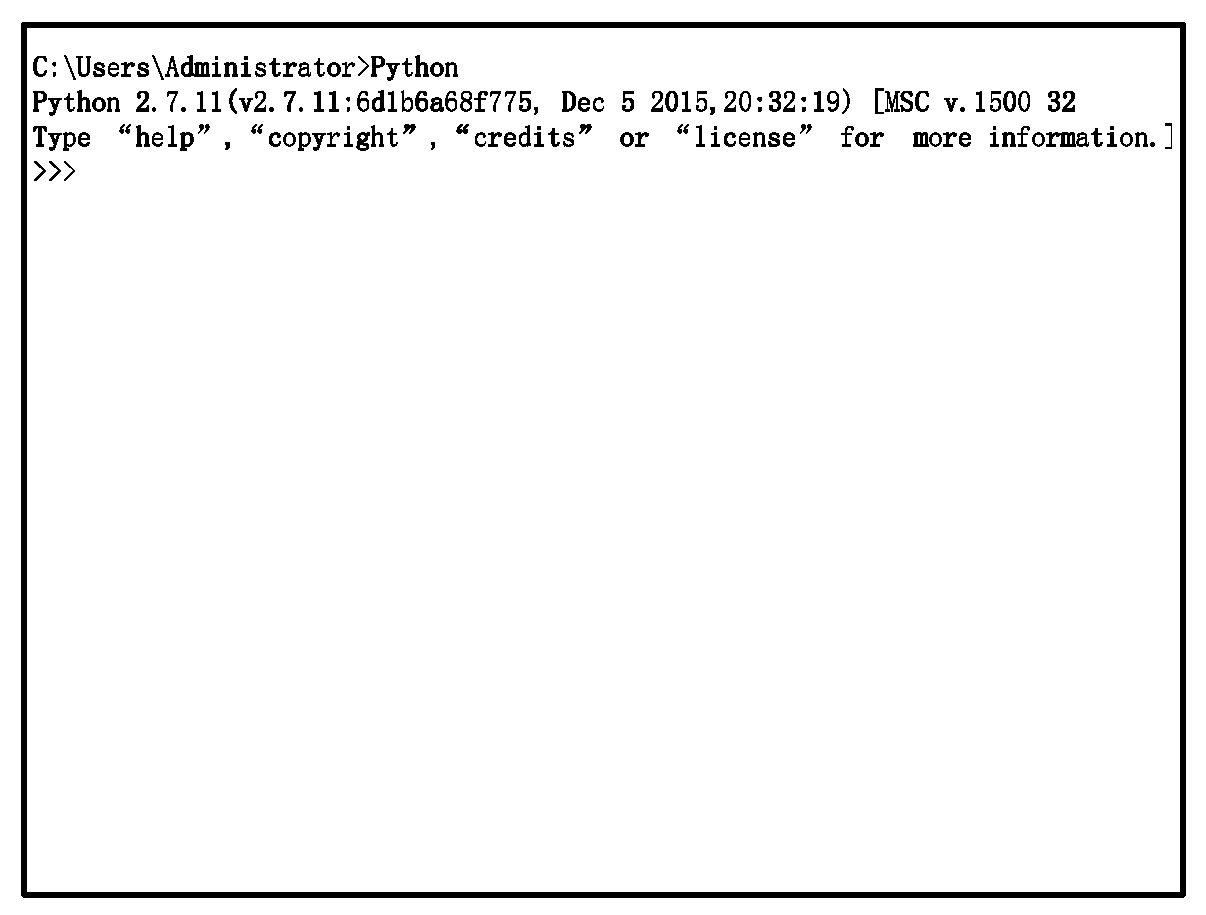
\includegraphics[width=10cm]{fig3_1}
%\caption{Python 安装勾选组件}
%\end{figure}
\begin{figure}[ht]
\centering
%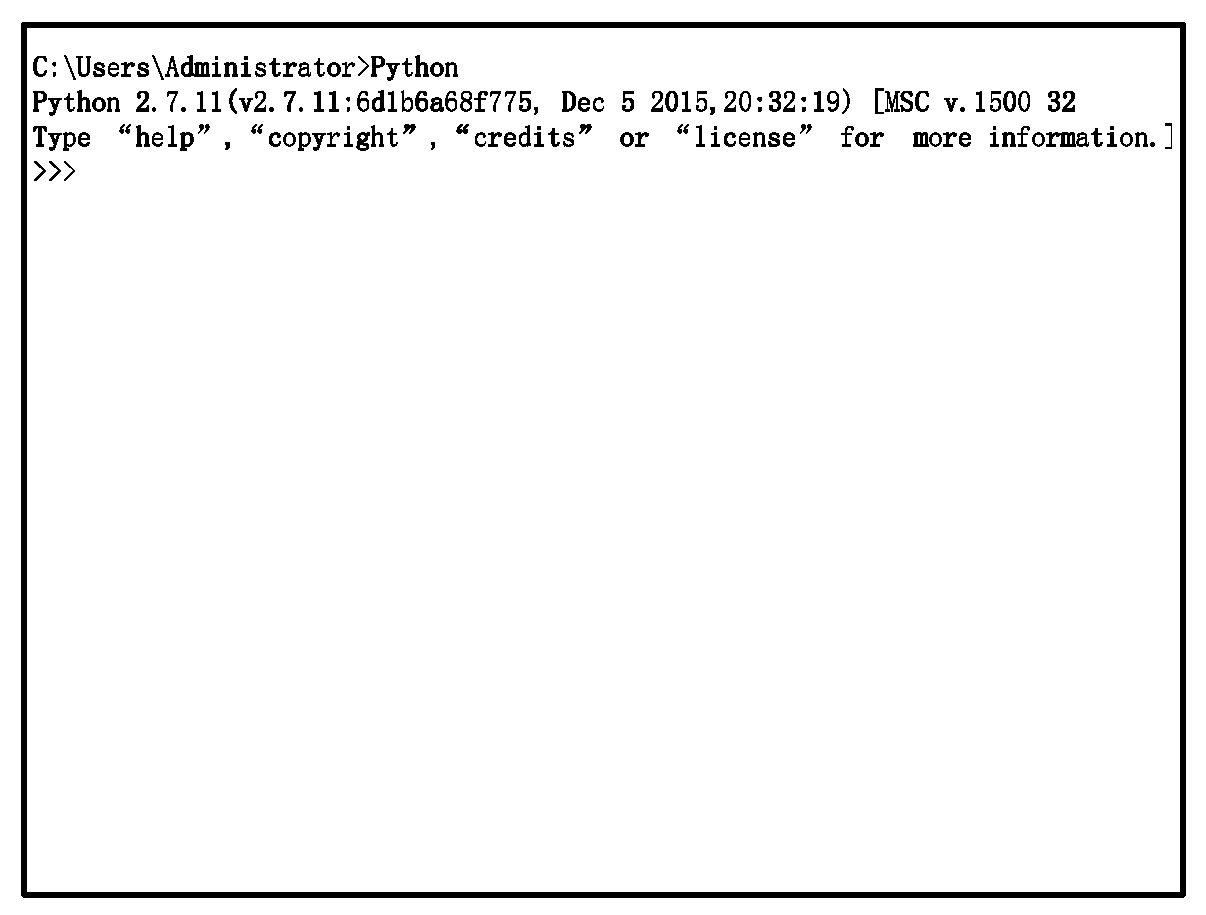
\includegraphics[width=9.6cm,height=7cm]{fig3_1}
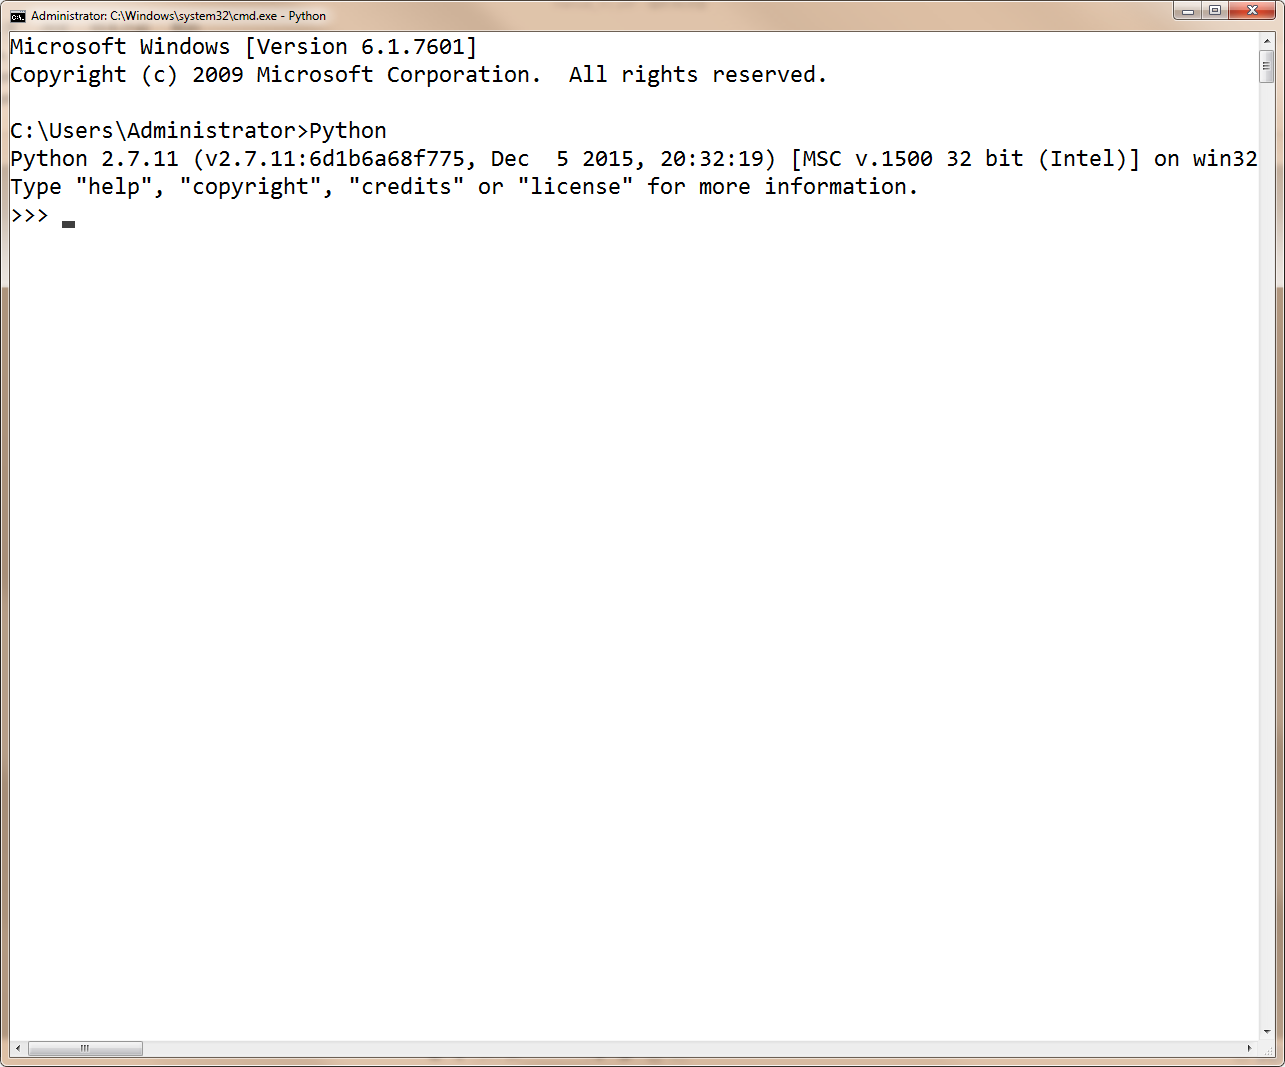
\includegraphics[height=7.5cm]{fig3_1_0}
\caption{\hspace{0.2cm}Python interpreter has been installed}
\end{figure}

\newpage
\section{\heiti Installing python packages}
\hspace{-0.2cm}We  provide all of the python packages required to run the software, such as wxpython, matplotlib, numpy and six. To install these packages, perform the following steps.
%我司会为用户提供运行软件所需的所有第三方Python库的安装文件,包括wxpython、matplotlib(包括dateutil文件与pyparsing文件)、numpy、six等。下面依次讲解如何安装这4个第三方库。
\vspace{0.3cm}

\noindent$\vcenter{\hbox{\huge$\bullet$}}$\quad\fontsize{12pt}{\baselineskip}\textbf{\heiti{Installing wxpython}}

\hspace{-0.2cm}You should open the `wxpython' folder in the `ASG\_install' folder, then double click the installation program and click `Next' will install this package.
%进入我司为用户提供的ASG\_install文件夹下的wxpython文件夹,双击其中的exe安装程序,点击“Next”即可安装wxpython库。
\vspace{0.3cm}

%\newpage
\noindent$\vcenter{\hbox{\huge$\bullet$}}$\quad\fontsize{12pt}{\baselineskip}\textbf{\heiti{Installing matplotlib} }

\hspace{-0.2cm}You should open the `matplotlib' folder in the `ASG\_install' folder, then double click the installation program and click `Next' will install this package.
%进入我司为用户提供的ASG\_install文件夹下的matplotlib文件夹,双击其中的exe安装程序,点击“Next” 即可安装matplotlib库。安装matplotlib库后还需要安装dateutil与pyparsing两个文件。
\vspace{0.3cm}

\noindent$\vcenter{\hbox{\huge$\bullet$}}$\quad\fontsize{12pt}{\baselineskip}\textbf{\heiti{Installing six}}

\hspace{-0.2cm}You should open the command window, then use `cd' command to switch the current directory as the location that you deposit the `six' folder. Then you can input `pip install six-1.10.0-py2.py3-none-any.whl' to install the package. For example, if user put `ASG\_install' folder in the root directory of  the E disk, the whole installation procedure will be shown in Fig 3.2 .
%在Windows命令窗口将目录切换到存放我司提供的six文件夹所在位置,然后通过“pip install”命令来安装six库。如用户将ASG\_install 文件夹放在E盘的主目录下,完整安装过程如图3.5。
\begin{figure}[H]
\centering
%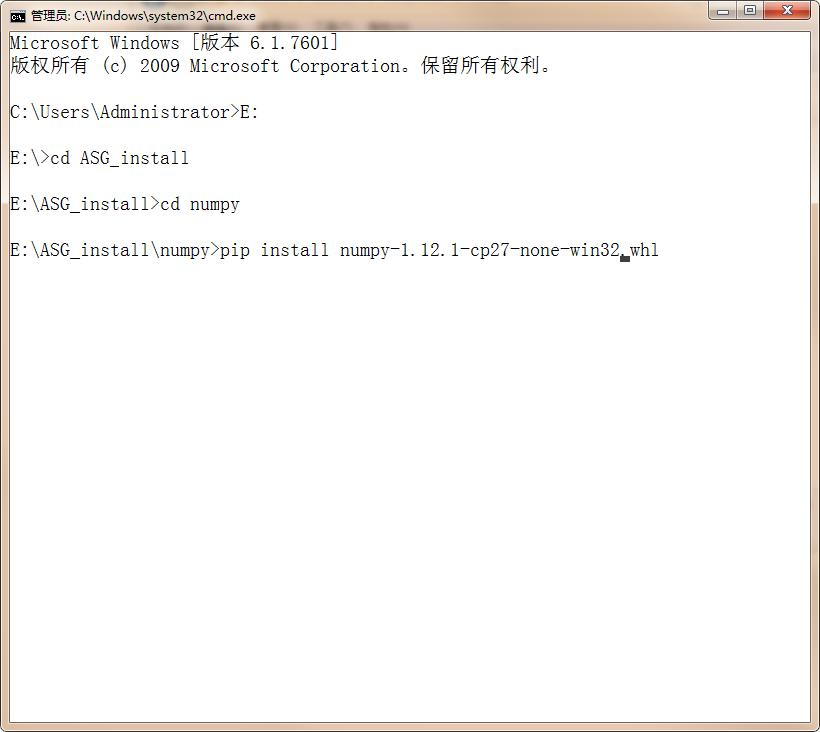
\includegraphics[width=9.6cm,height=7cm]{fig3_5}
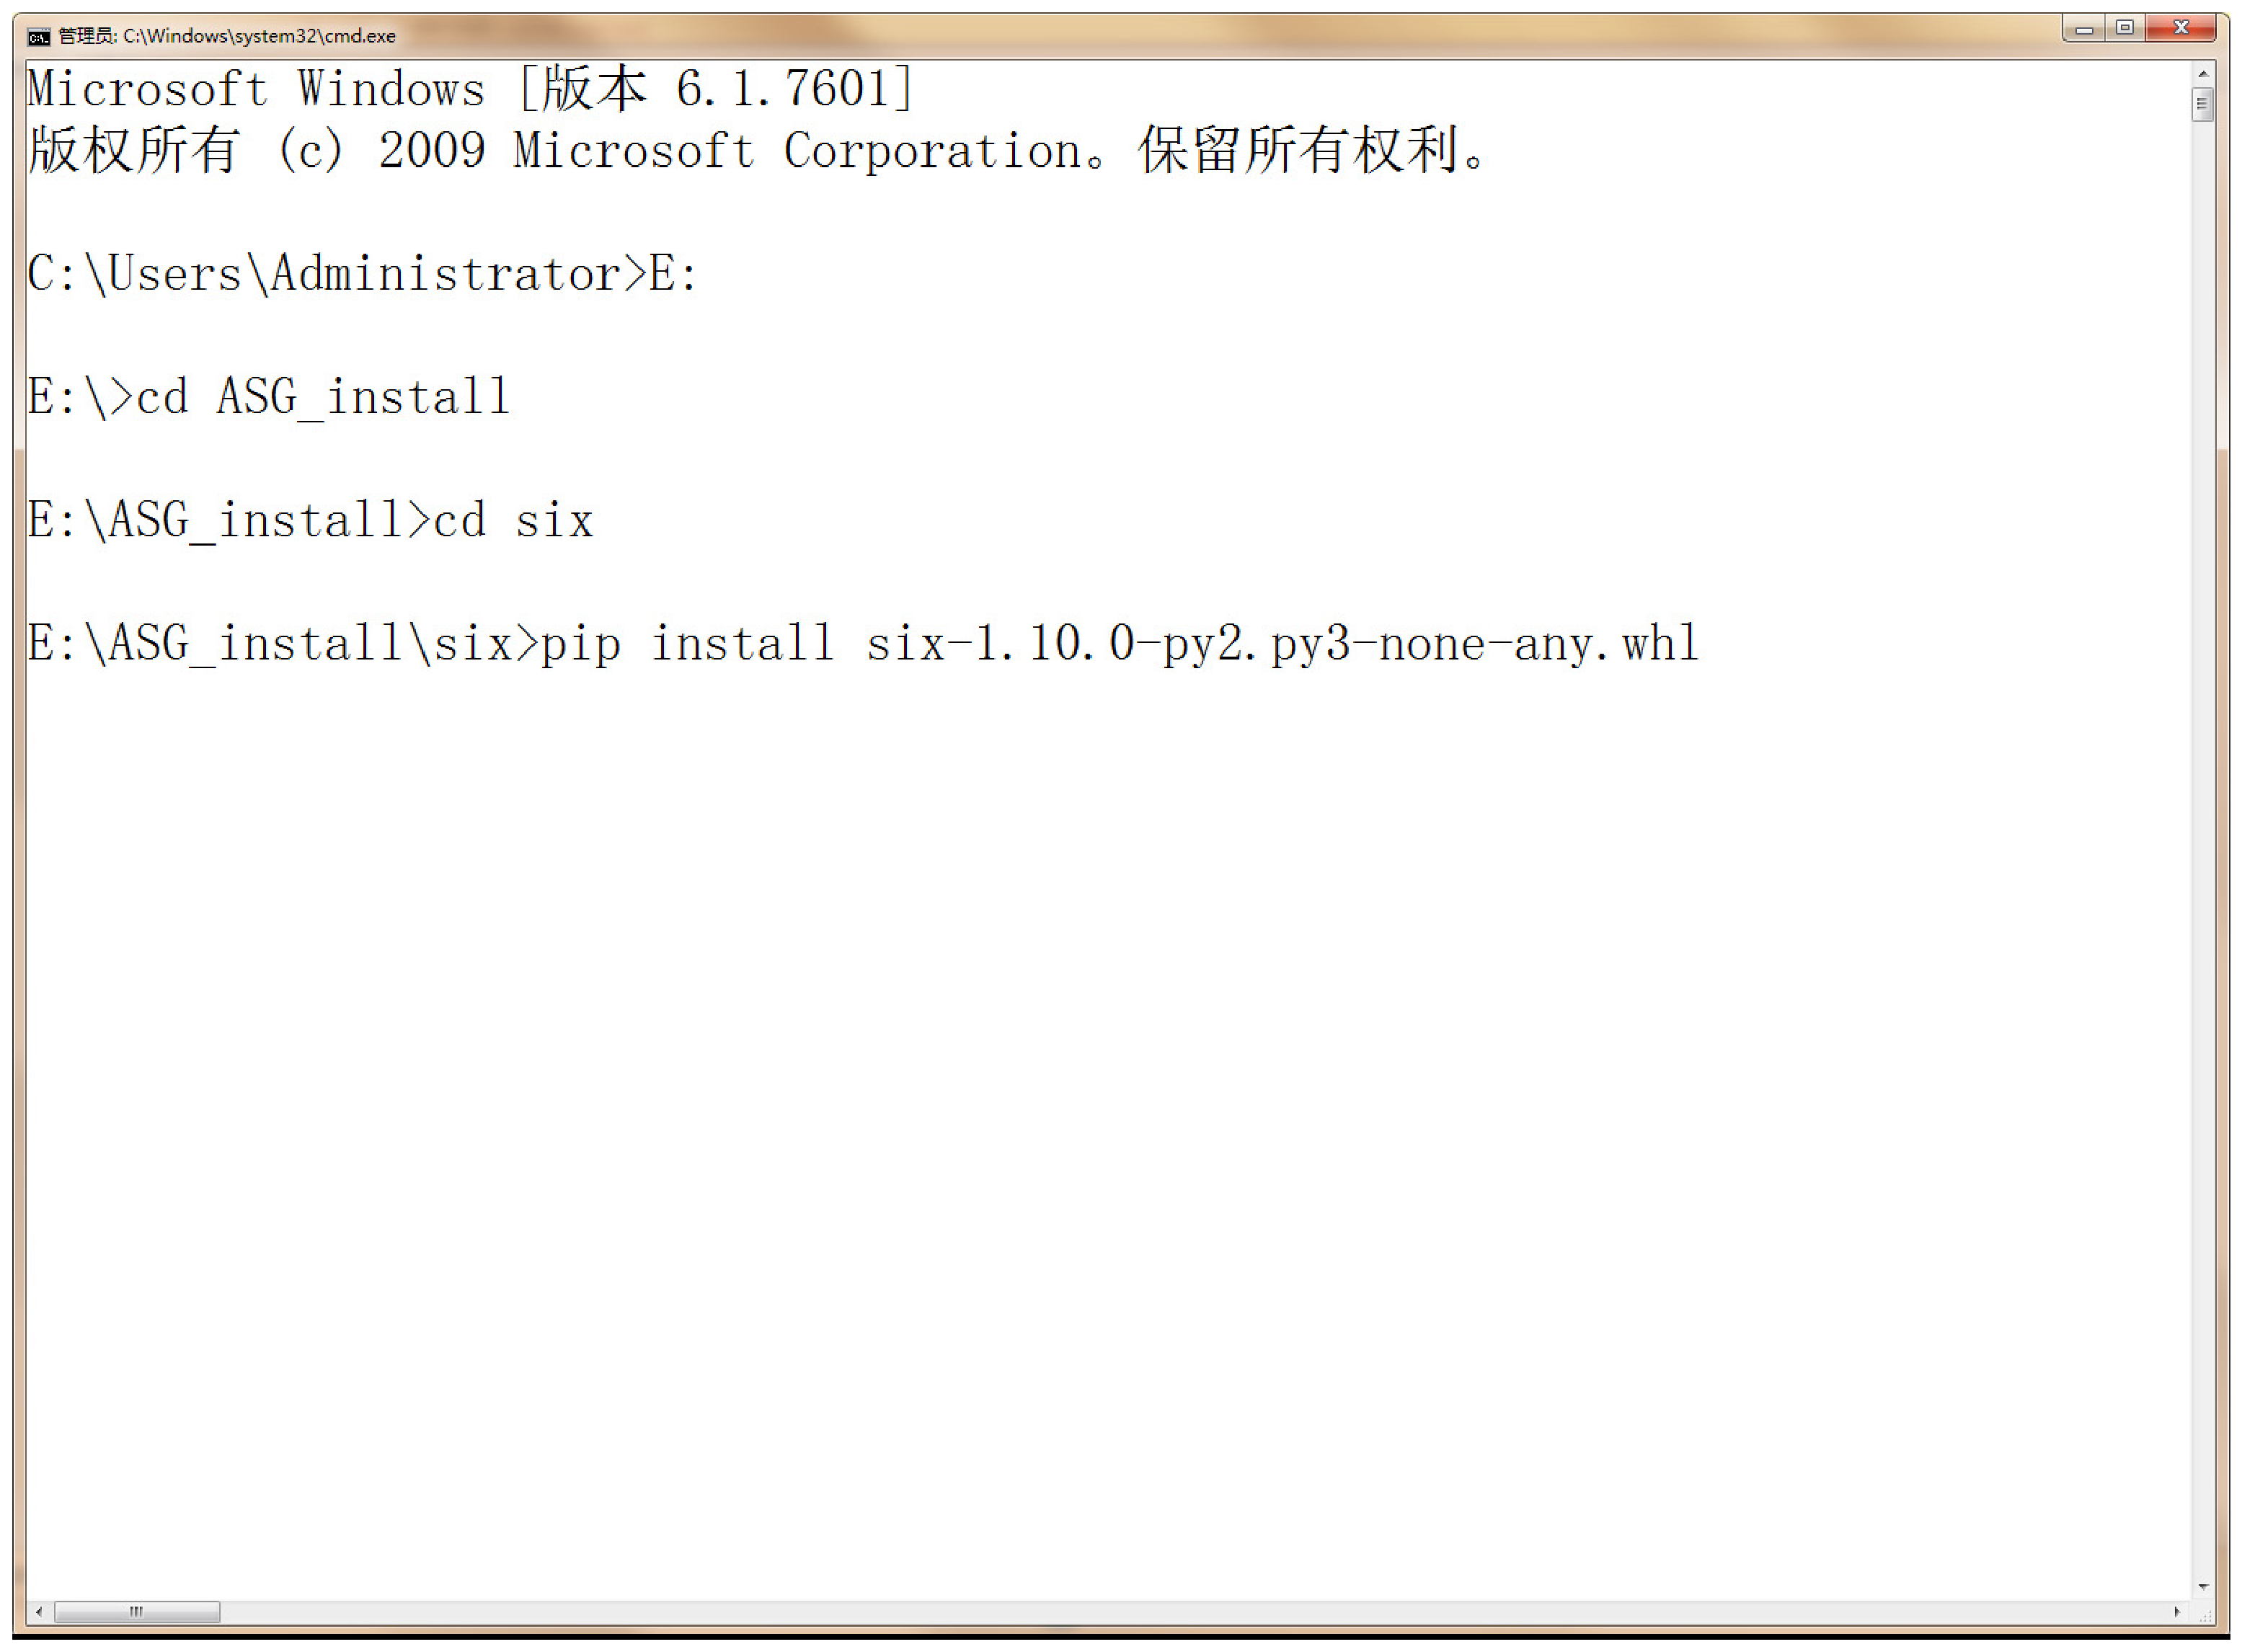
\includegraphics[height=7.5cm]{fig3_5_0}
\caption{\hspace{0.2cm}Installing six}
\end{figure}

%\newpage
\noindent$\vcenter{\hbox{\huge$\bullet$}}$\quad\fontsize{12pt}{\baselineskip}\textbf{\heiti{Installing dateutil} }

\hspace{-0.2cm}You should open the command window, then use `cd' command to switch the current directory as the location that you deposit the `matplotlib' folder. For example, if user put the `ASG\_install' folder in the root director of E disk, please input `E:' → `cd ASG\_install' → `cd matplotlib', then input `pip install python\_dateutil-2.6.0-py2.py3-none-any.whl' to install file dateutil. The whole installation procedure will be shown in Fig 3.3 .
%进入Windows命令窗口(点击任务栏“开始”→“运行”,在弹出窗口中输入“cmd”后点击“确定”),然后使用“cd”命令将当前目录切换到您存放我司提供的matplotlib文件夹所在位置。如用户将ASG\_install文件夹放在E 盘的主目录下,在命令窗口中依次输入“E:” → “cd ASG\_install” → “cd matplotlib”,即可将当前目录切换到存放matplotlib文件夹的位置。然后通过“pip install python\_dateutil-2.6.0-py2.py3-none-any.whl” 命令安装dateutil 文件。完整过程为如图3.2,依次输入命令即可安装dateutil 文件。
\begin{figure}[ht]
\centering
%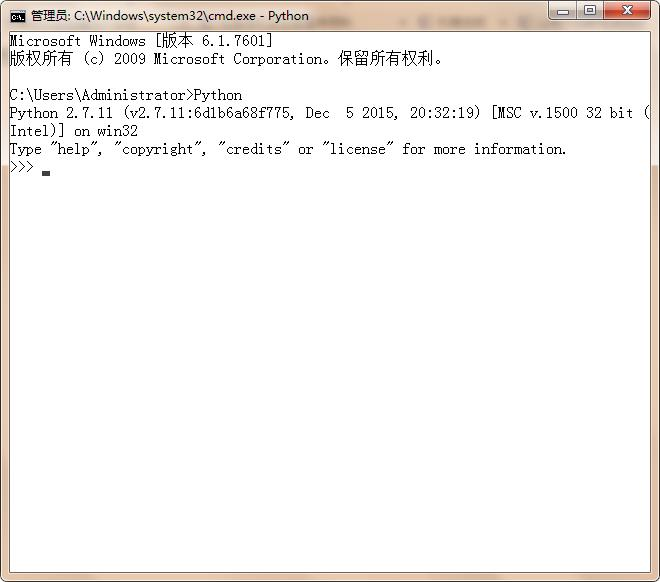
\includegraphics[width=9.6cm,height=7cm]{fig3_2}
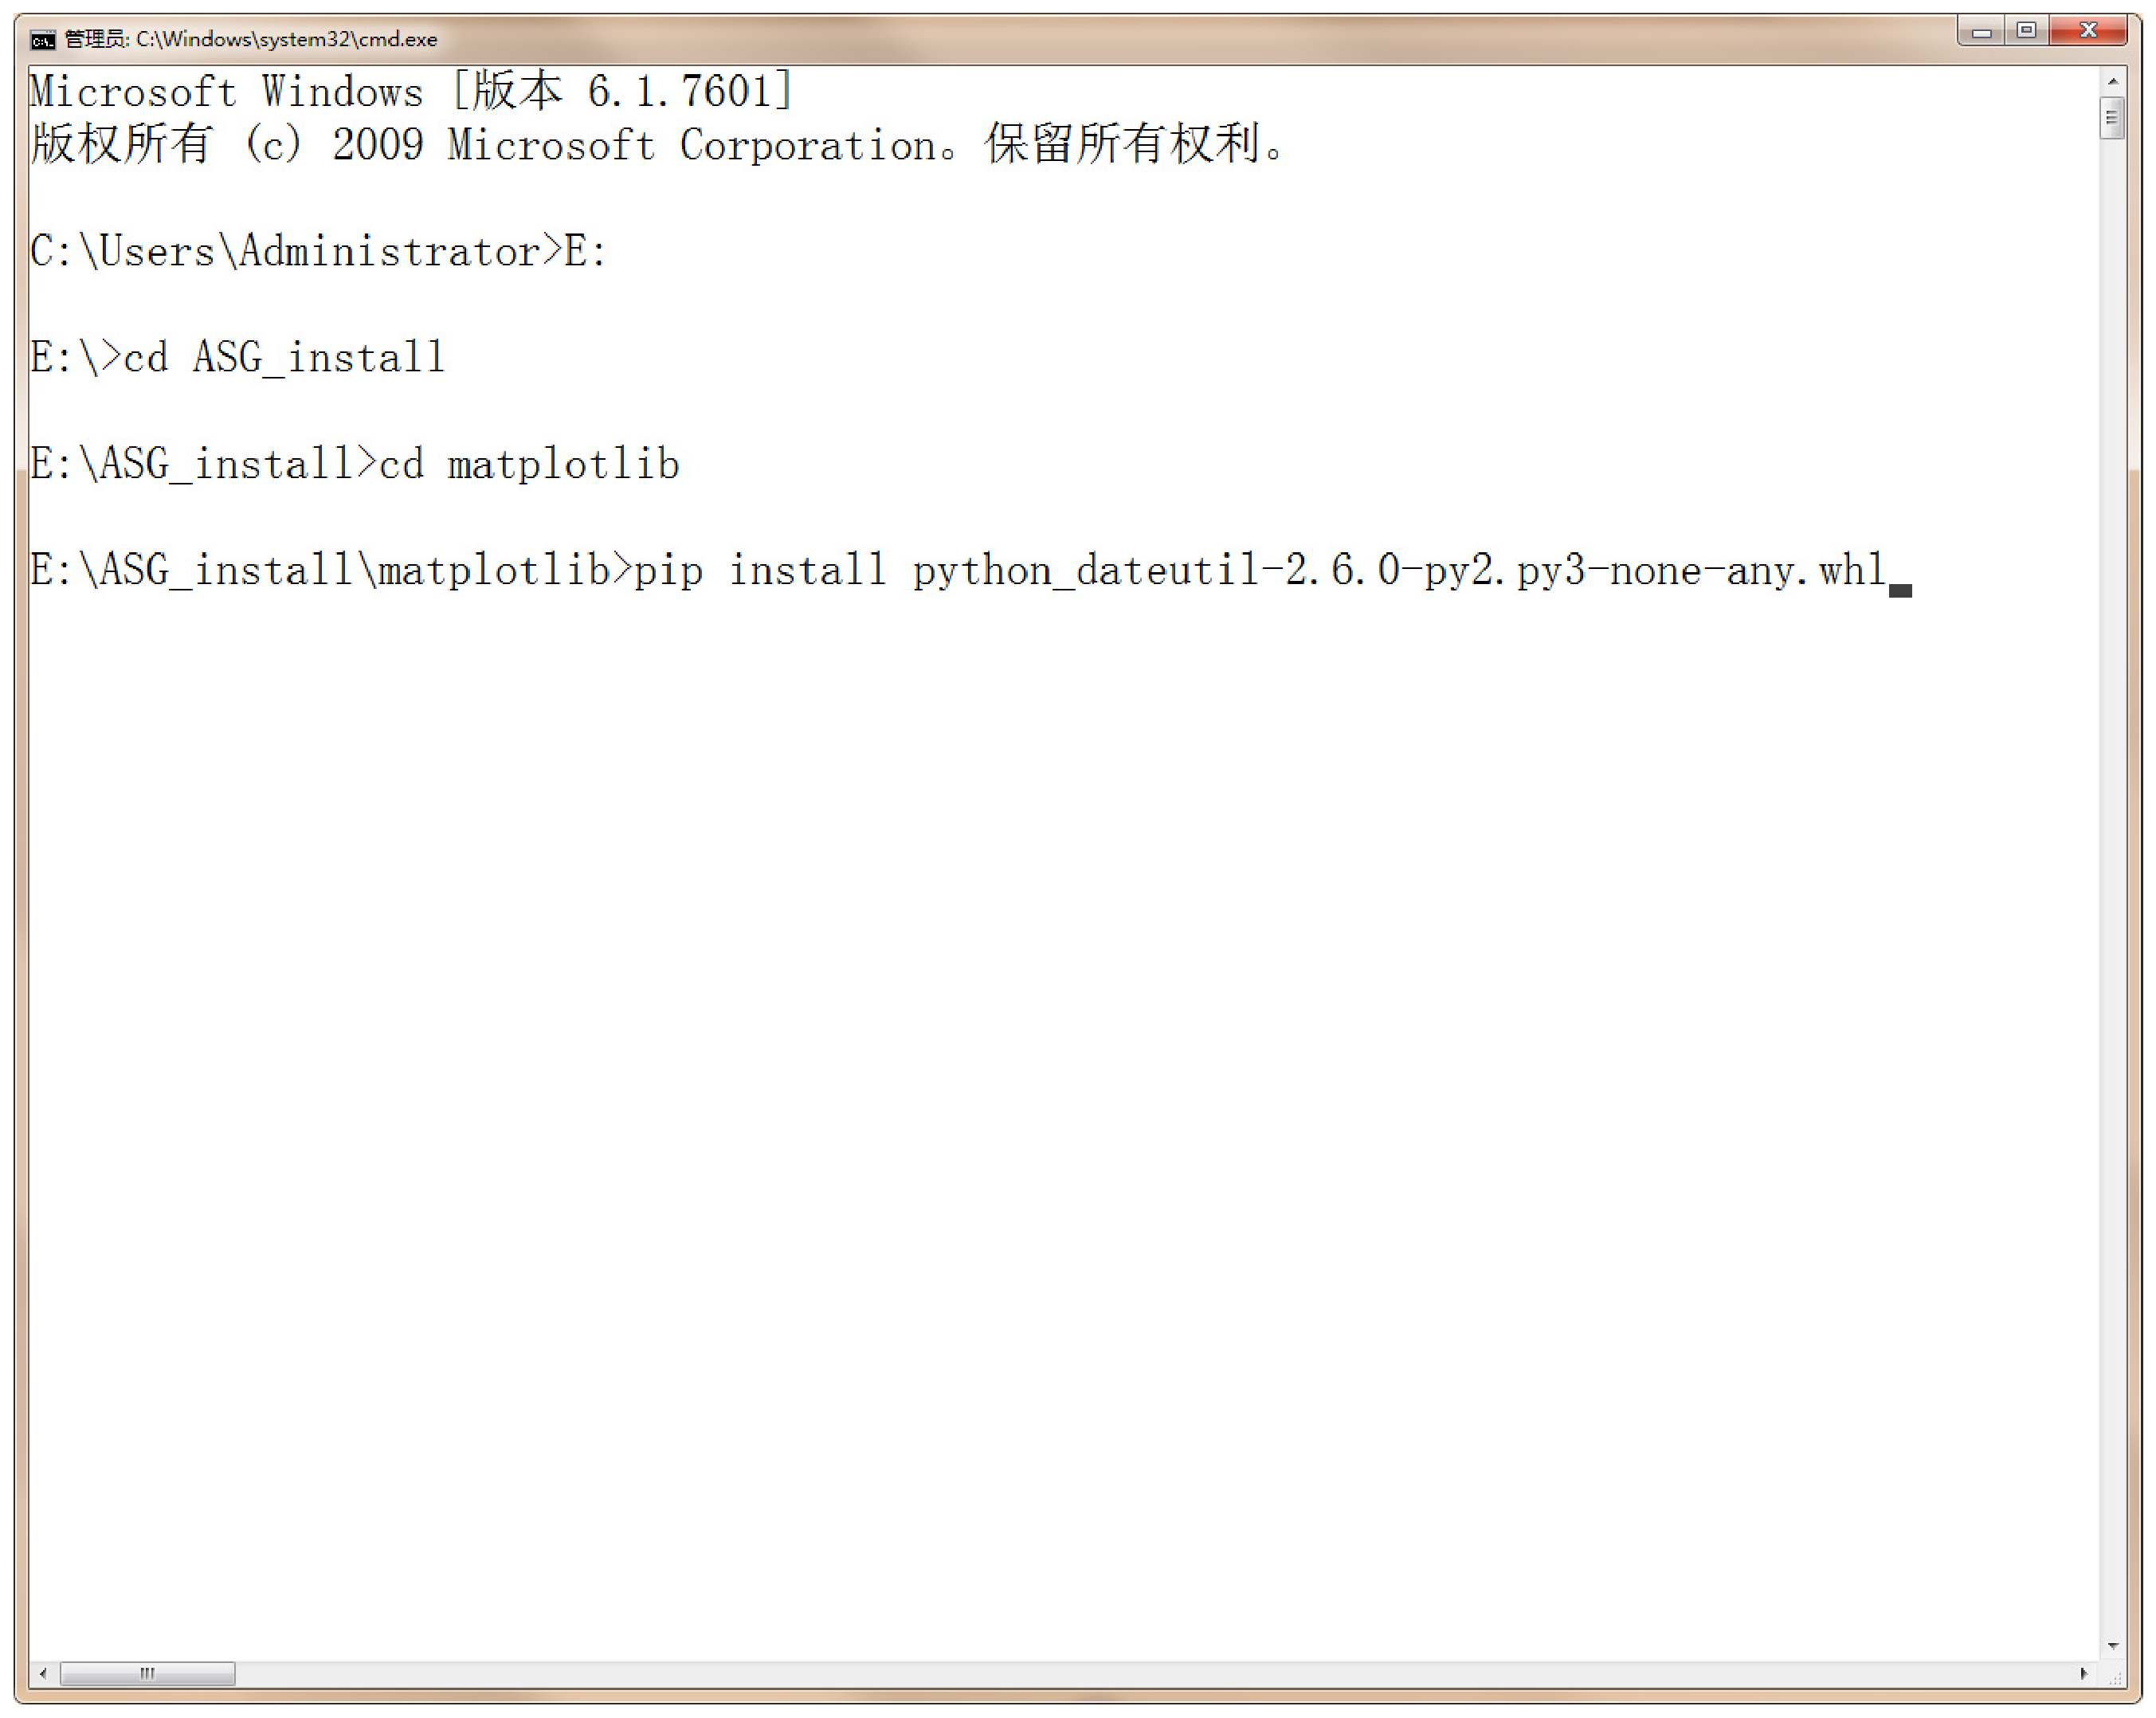
\includegraphics[height=7.5cm]{fig3_2_0}
\caption{\hspace{0.2cm}Installing dateutil}
\end{figure}

\noindent$\vcenter{\hbox{\huge$\bullet$}}$\quad\fontsize{12pt}{\baselineskip}\textbf{\heiti{Installing pyparsing}}

\hspace{-0.2cm}As the installation steps of dateutil file, switch the current directory as the location that you deposit the the `matplotlib' folder. Then input `pip install pyparsing-2.2.0-py2.py3-none-any.whl' to install file pyparsing. For example, if user put `ASG\_install' folder in the root directory of E disk, the whole installation procedure will be shown in Fig 3.4 .
%同安装dateutil文件一样,在Windows命令窗口将目录切换到我司提供的matplotlib文件夹所在位置,然后通过“pip install pyparsing-2.2.0-py2.py3-none-any.whl”命令安装pyparsing文件。如用户将ASG\_install 文件夹放在E 盘的主目录下,完整安装过程如图3.3。

%进入Windows命令行,然后将目录切换到您存放我司提供的“matplotlib”文件夹所在位置。如图3-3输入命令即可安装pyparsing文件。

\begin{figure}[H]
\centering
%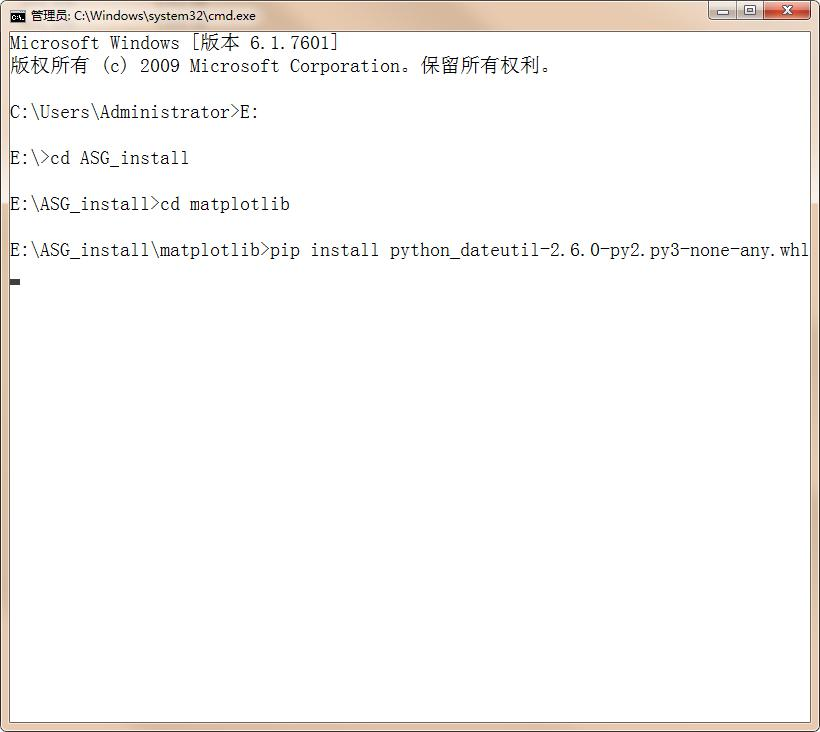
\includegraphics[width=9.6cm,height=7cm]{fig3_3}
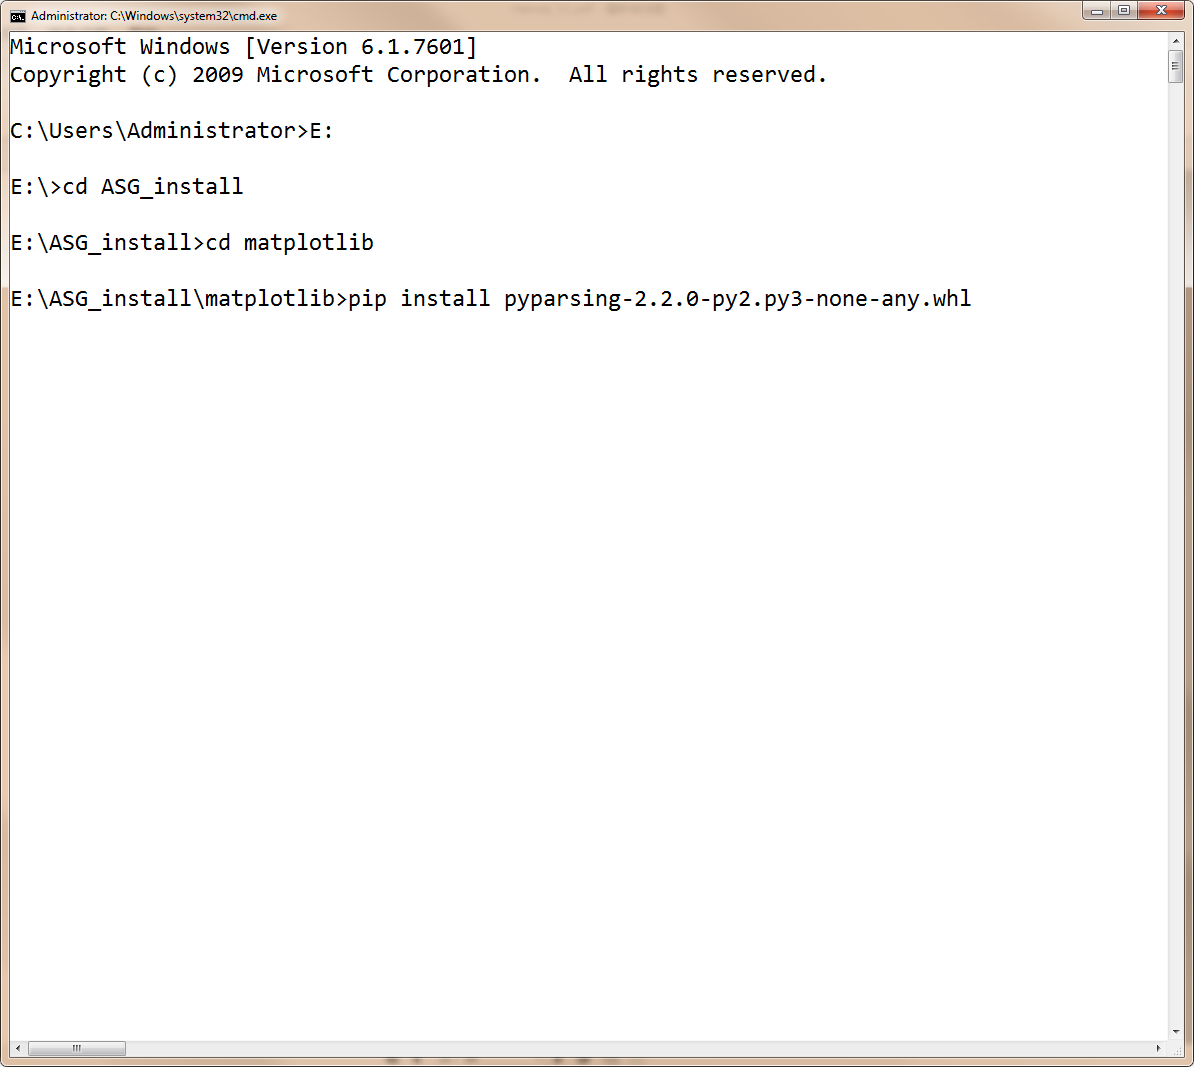
\includegraphics[height=7.2cm]{fig3_3_0}
\caption{\hspace{0.2cm}Installing pyparsing}
\end{figure}

\noindent$\vcenter{\hbox{\huge$\bullet$}}$\quad\fontsize{12pt}{\baselineskip}\textbf{\heiti{Installing numpy}}

\hspace{-0.2cm} You should open the command window and switch the current directory as the location that you deposit the `numpy' folder, then input `pip install numpy-1.12.1-cp27-none-win\_amd32.whl' to install the package. For example, if user put `ASG\_install' folder in the root directory of E disk, the whole installation procedure will be shown in fig 3.5 .
%在Windows命令窗口将目录切换到存放我司提供的numpy文件夹所在位置,然后通过“pip install numpy-1.12.1-cp27-none-win\_amd32.whl”命令安装numpy库。如用户将ASG\_install文件夹放在E盘的主目录下,完整安装过程如图3.4。
\begin{figure}[H]
\centering
%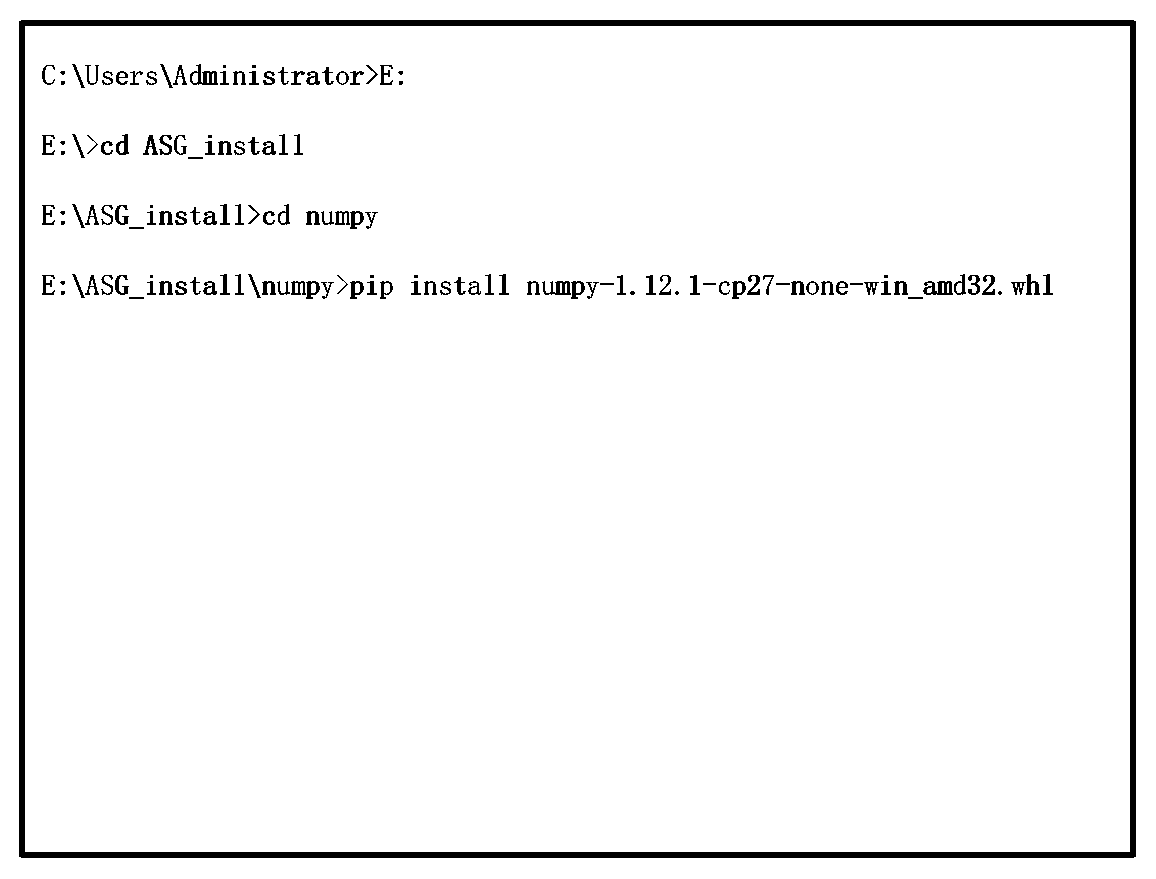
\includegraphics[width=9.6cm,height=7cm]{fig3_4}
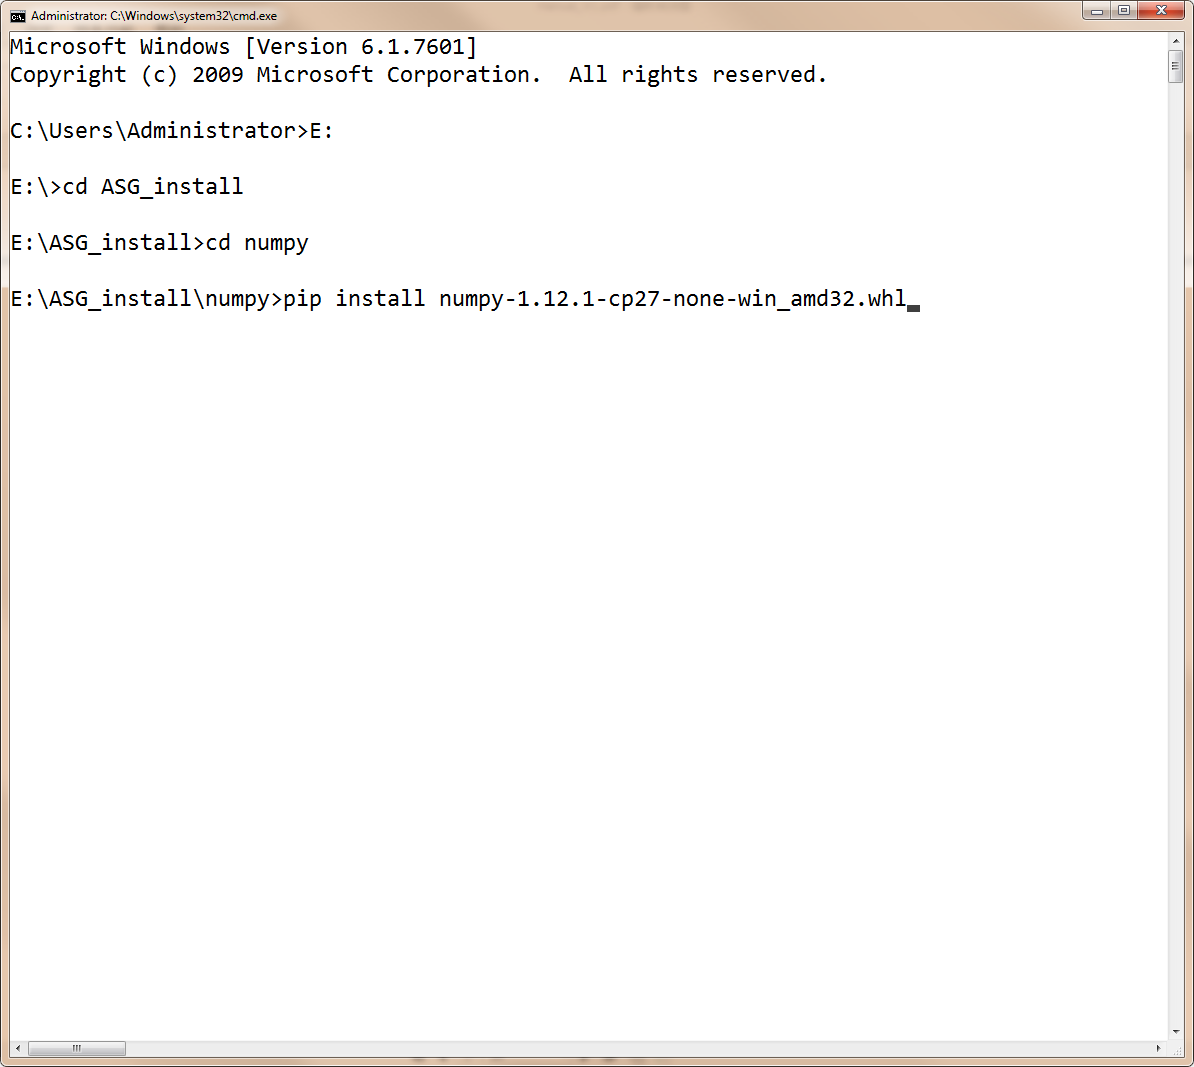
\includegraphics[height=7.2cm]{fig3_4_0}
\caption{\hspace{0.2cm}Installing numpy}
\end{figure}

\vspace{0.8cm}
\section{\heiti Installing USB driver program}

\hspace{-0.2cm}When a computer connect to the product for the first time, the USB driver program will be installed automatically. Right click `Computer'→`manage'→`Device Manager', if you find `EZ-USB FX2 GPIF to Ext FIFO Example using Single Transactions' in `Universal Serial Bus controllers', you need to install the program manually. Please right click `EZ-USB FX2 GPIF to Ext FIFO Example using Single Transactions'→`Update Driver Software'→`Browse my computer for driver software', then switch current directory as the location that you deposit the `Drivers' folder in `ASG\_install' folder. If the program has been installed successfully, you will see that `Cypress FX3 USB StreamerExample Device' has been recognized as Fig 3.6.
%在一台计算机上首次连接产品时,系统会自动安装产品运行所需的USB驱动程序。请右键“计算机”→“管理”,点击“设备管理器”,查看USB 驱动程序安装是否成功。若在“通用串行总线控制器”找到驱动未安装成功的设备中有“EZ-USB FX2 GPIF to Ext FIFO Example using Single Transactions”一项,则需要手动安装驱动程序(右键选择该设备→ 更新驱动程序软件→浏览计算机以查找驱动程序软件),选择目录至我司为用户提供的“ASG\_install” 文件夹下的“Drivers” 文件夹即可。驱动安装成功后,在设备管理器中可以看到如图3.6 所示的“Cypress FX3 USB StreamerExample Device” 被识别的状态。
\begin{figure}[htbp]
\centering
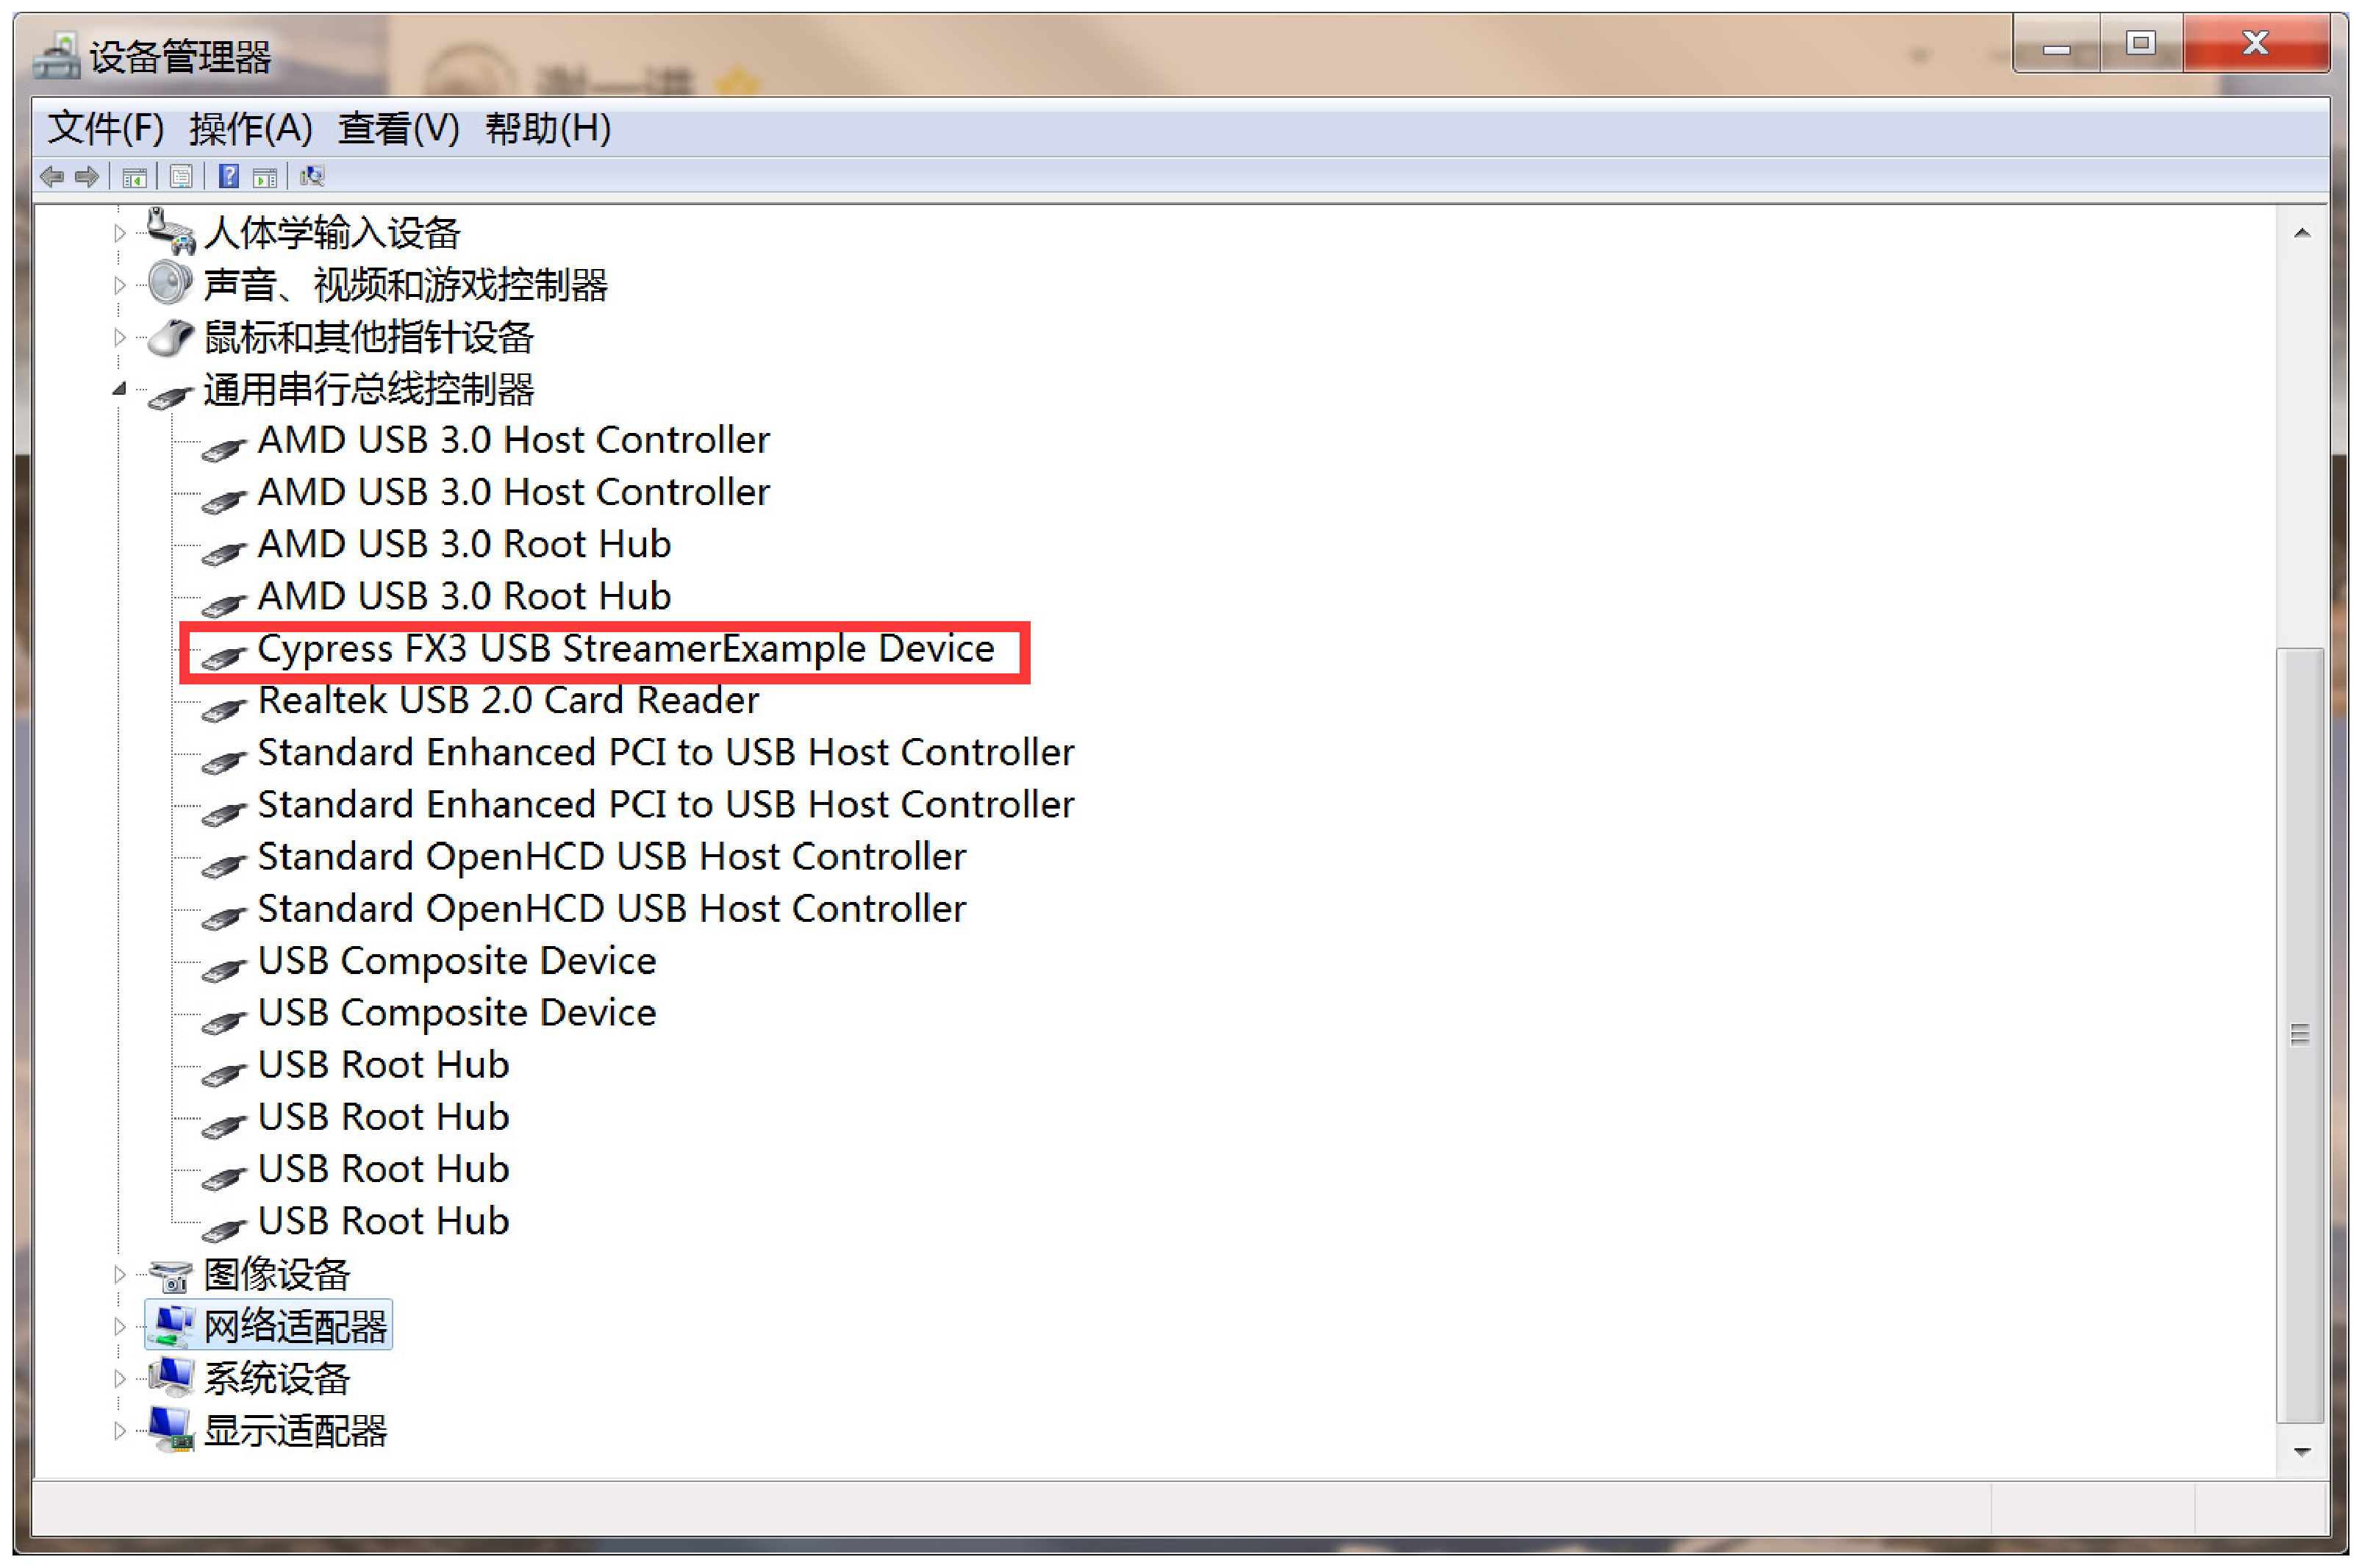
\includegraphics[width=10cm,height= 9.0cm]{fig3_6}
%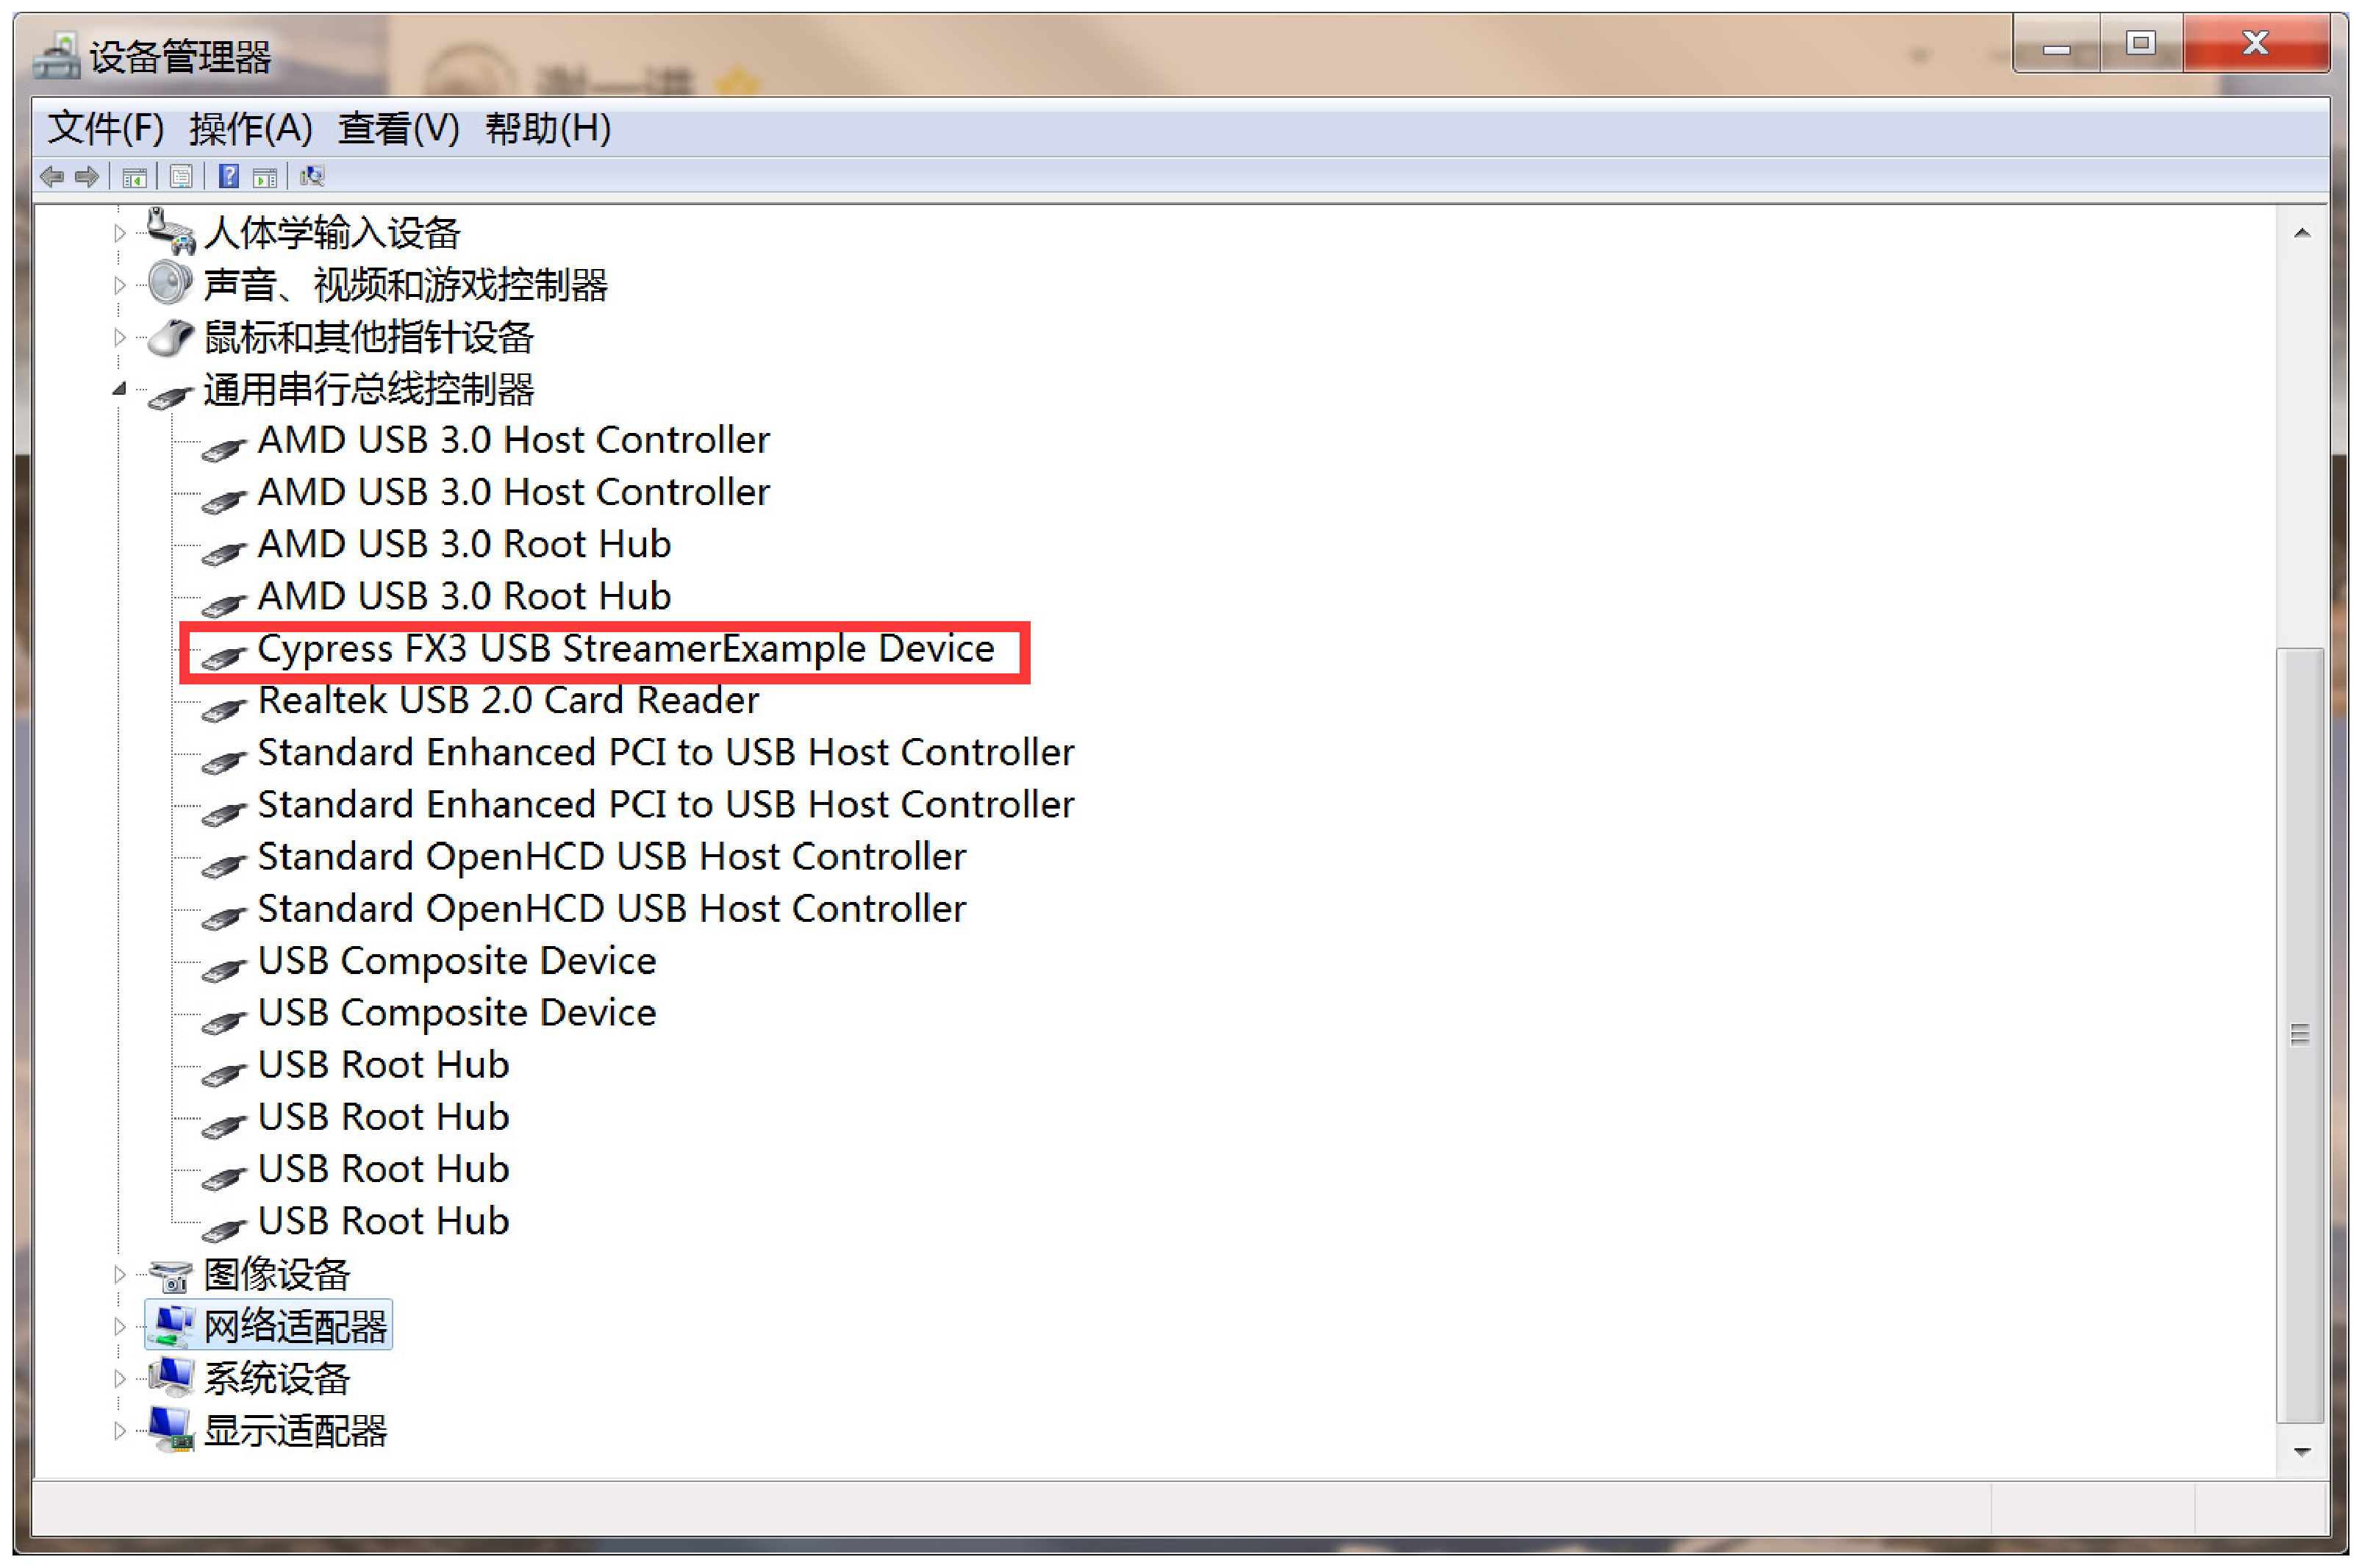
\includegraphics[height= 8.0cm]{fig3_6}
\caption{\hspace{0.2cm}Installing USB driver}
\end{figure}

\hspace{-0.2cm}When the USB driver program has been installed, right click `Cypress FX3 USB StreamerExample Device'→`Properties'→`Power Management', please uncheck the selection as Fig 3.7.
%驱动程序安装完成后,双击“Cypress FX3 USB StreamerExample Device”打开其属性,进入“电源管理”选项。如图3.7,取消勾选“允许计算机关闭此设备以节约电源”。
\begin{figure}[htbp]
\centering
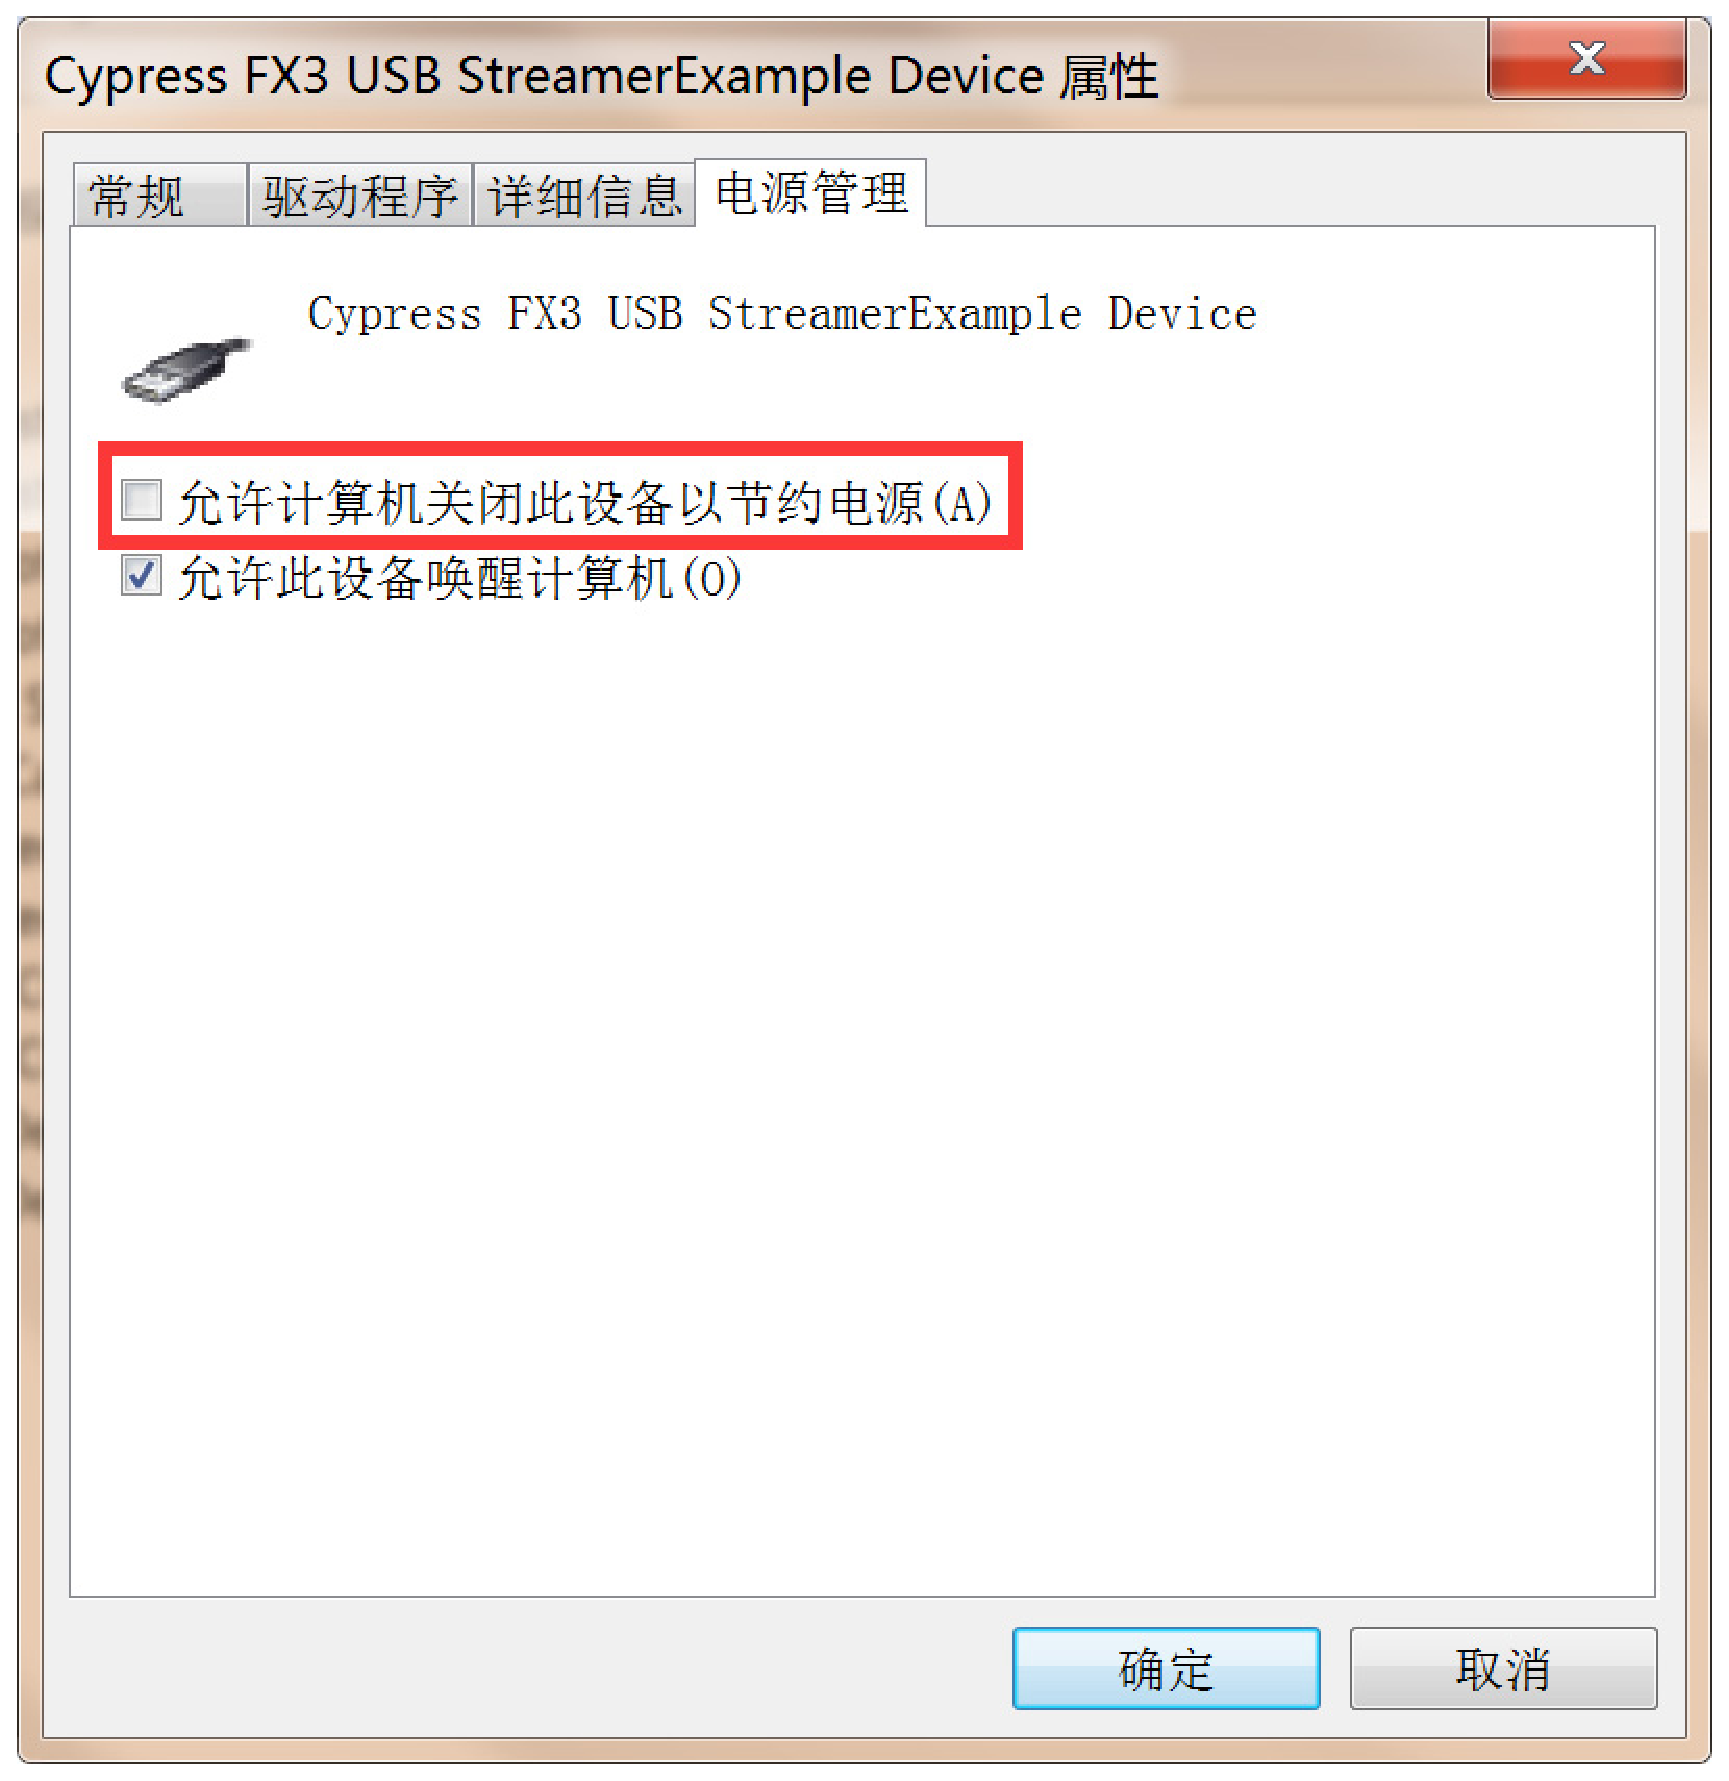
\includegraphics[width=10cm,height=9.5cm]{fig3_7}
%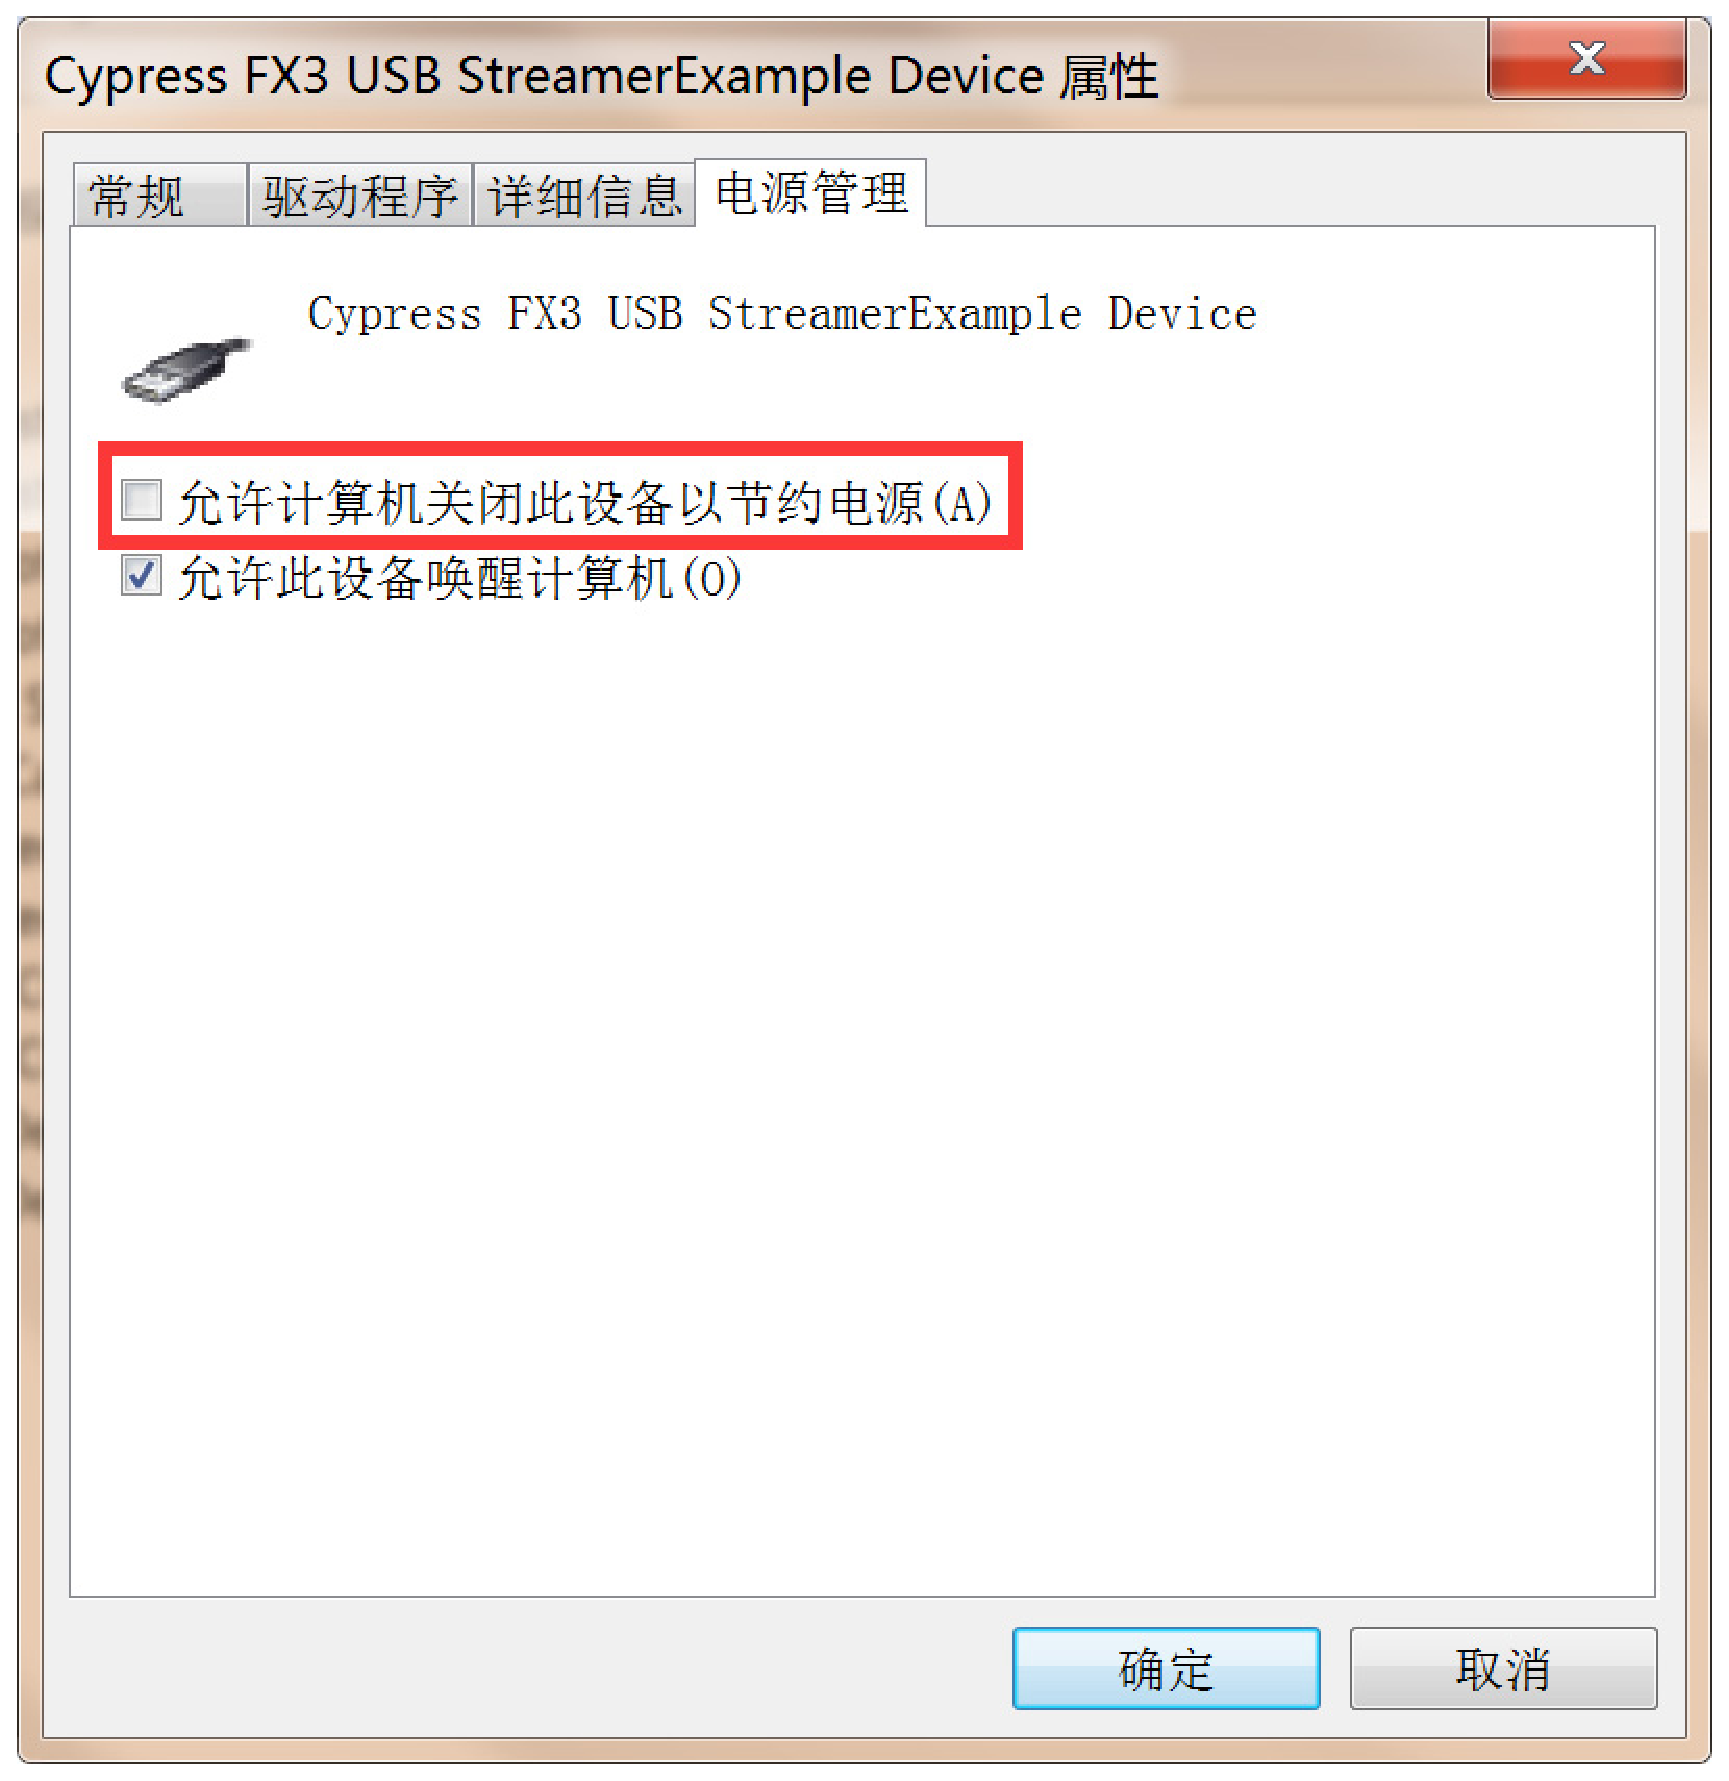
\includegraphics[height=9.0cm]{fig3_7}
\caption{\hspace{0.2cm}Uncheck power manager}
\end{figure}
